% =====================================================================
%  IN6049 --- Forecasting and Regression Analysis
%  Week 9: Introduction to Forecasting and Statistics Background --- Airline passengers
%
%  Built from template/slides-template.tex (Boadilla + seahorse, 16:9).
%  Title slide + 9 content slides.  Numbers come from Assigment_9.ipynb;
%  figures are its exported PNGs (images/ -> fig_*.png here).
%
%  Compiles on Overleaf with the default pdfLaTeX engine.
%  Upload alongside: fig_ts.png , fig_forecast.png , fig_filters.png ,
%  fig_acf.png , fig_boxcox.png , fig_decomp.png , fig_errdiag.png , fig_control.png
% =====================================================================
\documentclass[aspectratio=169,11pt]{beamer}

\usetheme{Boadilla}
\usecolortheme{seahorse}
\setbeamertemplate{navigation symbols}{}

\usepackage[utf8]{inputenc}
\usepackage[T1]{fontenc}
\usepackage{booktabs}
\usepackage{amsmath}
\usepackage{graphicx}
\usepackage{url}

% Emphasis lead-in: bold + structure colour.  Use as \key{Finding.} text...
\newcommand{\key}[1]{\textbf{\structure{#1}}}

% Figure placeholder, so the template compiles with no image files.
% Replace each use by  \includegraphics[width=0.9\linewidth]{@@ file @@}
% (vector PDF preferred; PNG is fine).
\newcommand{\figbox}[2]{%
  \fbox{\parbox[c][#2][c]{#1}{\centering\scriptsize\color{gray}@@ figure @@}}}

% ---------------------------------------------------------------------
\title[Forecasting and statistics background]{Introduction to Forecasting and Statistics Background}
\subtitle{Monthly airline passengers, 1949--1960}
\author[Jie Dong, Elivier Reyes]{Jie Dong, Elivier Reyes}
\date[IN6049]{}

\begin{document}

% ===================== TITLE ========================================
\begin{frame}
  \titlepage
  \vspace{-1.2em}
  \begin{center}
    \small\urlstyle{same}\url{https://github.com/HelloJJJie/Assignment-Forecast-and-Analysis-of-Regression.git}

    \vspace{1.2em}
    $T=144$ monthly observations: what can we say about the next ones,
    and how sure can we be?
  \end{center}
\end{frame}

% ===================== 1. FROM REGRESSION TO TIME SERIES ============
\begin{frame}{1. From regression to time series, and the data}
  \begin{columns}[T]
  \begin{column}{0.50\textwidth}
    \small
    \key{What changes.} The rows of \texttt{tips.csv} had no order; in a time
    series the order is part of the data: neighbouring values are correlated,
    validation must respect time (no random splits), and the series is usually
    \emph{not} stationary.

    \vspace{0.3em}
    \key{Data.} Monthly airline passengers (thousands), Jan 1949--Dec 1960,
    $T=144$, no gaps; supplied by the course team, matching the classic
    Box--Jenkins series. Mean $280.3$, min $104$ (Nov 1949), max $622$ (Jul 1960).

    \vspace{0.3em}
    \key{Patterns:} an upward \emph{trend}, a yearly \emph{seasonal} cycle, and
    swings that \emph{grow with the level}.
  \end{column}
  \begin{column}{0.50\textwidth}
    \centering
    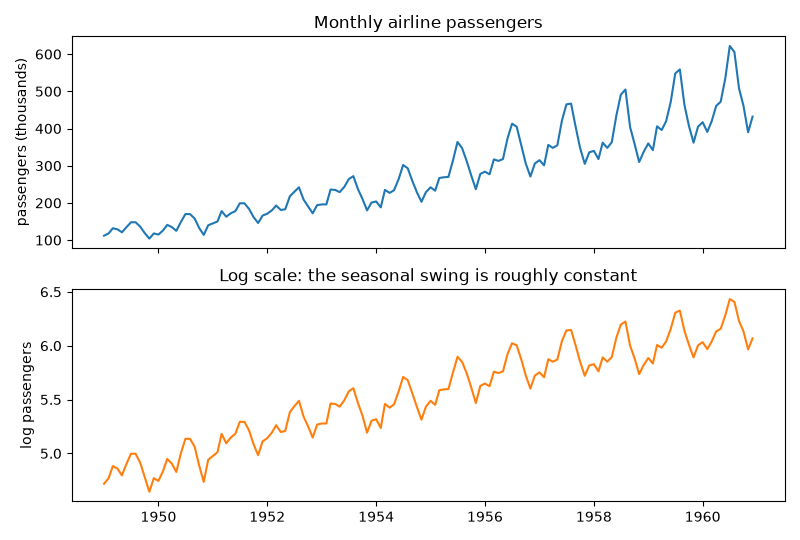
\includegraphics[width=0.92\linewidth]{fig_ts.png}
  \end{column}
  \end{columns}
\end{frame}

% ===================== 2. FORECASTS ================================
\begin{frame}{2. What is a forecast? Benchmarks and interval forecasts}
  \begin{columns}[T]
  \begin{column}{0.52\textwidth}
    \small
    $\hat y_{T+\tau}$ is made at the \emph{origin} $T$ for \emph{horizon}
    $\tau$. A point forecast is one number; an interval forecast shows the
    uncertainty, and it widens with $\tau$.

    \vspace{0.3em}
    \key{Benchmarks.} Lecture example (42, 45, 43, 47, 46, 49): naive $=49$,
    average $=45.3$. Airline, origin Dec 1959, all of 1960 held out:

    \vspace{0.2em}
    {\scriptsize
    \begin{tabular}{@{}lrrr@{}}
      \toprule
       & MAD & RMSE & MAPE \% \\
      \midrule
      mean            & $213.7$ & $226.3$ & $43.6$ \\
      naive           & $76.0$  & $103.0$ & $14.3$ \\
      seasonal naive  & $47.8$  & $50.7$  & $10.0$ \\
      drift           & $66.3$  & $92.7$  & $12.4$ \\
      \bottomrule
    \end{tabular}}

    \vspace{0.3em}
    The seasonal naive forecast ($y_{t-12}$) is the best simple rival: the
    series is dominated by its season.
  \end{column}
  \begin{column}{0.48\textwidth}
    \centering
    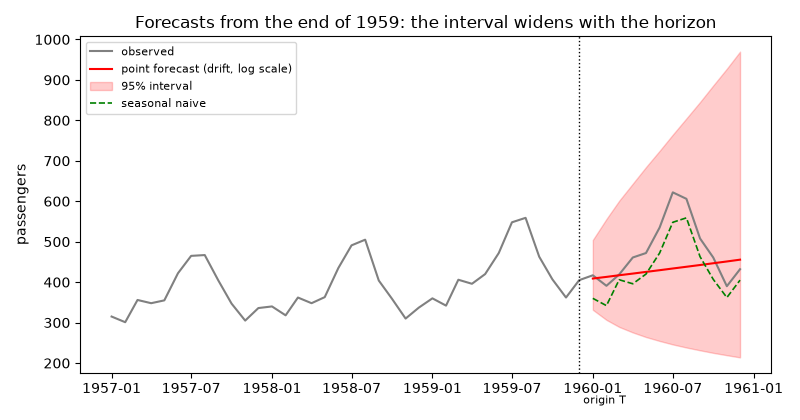
\includegraphics[width=0.92\linewidth]{fig_forecast.png}

    \vspace{-0.1em}
    \raggedright\scriptsize
    Random walk with drift on the log scale (an illustration, not a
    recommended model): the $95\%$ interval is $173$ wide at $\tau=1$ and
    $756$ at $\tau=12$; the actual 1960 values all fall inside.\par
  \end{column}
  \end{columns}
\end{frame}

% ===================== 3. ERRORS AND SMOOTHING ======================
\begin{frame}{3. Forecast errors vs.\ residuals, and smoothing}
  \begin{columns}[T]
  \begin{column}{0.46\textwidth}
    \small
    \key{Forecast error} $e_t(t-\tau)=y_t-\hat y_t(t-\tau)$ is out of sample;
    a \key{residual} $e_t=y_t-\hat y_t$ is in sample. Model: $\ln y_t=$ linear
    trend $+$ monthly indicators ($p=13$), fitted to the first $120$ months:

    \vspace{0.2em}
    {\scriptsize
    \begin{tabular}{@{}lr@{}}
      \toprule
      residual $s$ (in sample)          & $0.0548$ \\
      one-step forecast RMSE, next $24$ & $0.0808$ \\
      ratio                             & $1.48$ \\
      \bottomrule
    \end{tabular}}

    \vspace{0.3em}
    Residuals understate the true forecast error.

    \vspace{0.3em}
    \key{Smoothing.} Moving average $Var(M)=\sigma^2/N$ (simulated:
    $0.1993$ for $N=5$, $0.2$ expected). Hanning:
    $0.25y_{t+1}+0.5y_t+0.25y_{t-1}$. A synthetic spike of $+300$ moves the
    $5$-term average by $+60$ but the $5$-term median by $+9$.
  \end{column}
  \begin{column}{0.54\textwidth}
    \centering
    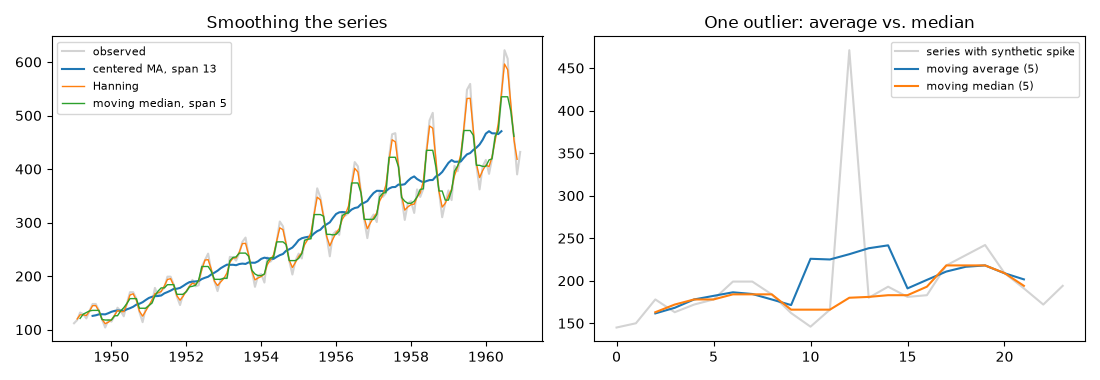
\includegraphics[width=0.98\linewidth]{fig_filters.png}
  \end{column}
  \end{columns}
\end{frame}

% ===================== 4. STATIONARITY AND ACF ======================
\begin{frame}{4. Stationarity and the autocorrelation function}
  \begin{columns}[T]
  \begin{column}{0.44\textwidth}
    \small
    $c_k=\frac1T\sum_{t=1}^{T-k}(y_t-\bar y)(y_{t+k}-\bar y)$, $r_k=c_k/c_0$,
    $se(r_k)=1/\sqrt T$; rules: $T\ge50$, $K\approx T/4$,
    significant if $|r_k|>2/\sqrt T$. Divisor $T$ (not $T-1$).

    \vspace{0.3em}
    \key{Checks.} Slide-10 series ($T=10$): $r_1,r_2,r_3=-0.79,\,+0.46,\,-0.16$,
    bound $\pm0.63$ (as in the lecture). Airline: $T=144$, $K=36$,
    bound $\pm0.167$.

    \vspace{0.3em}
    \small
    {\scriptsize\setlength{\tabcolsep}{2pt}
    \begin{tabular}{@{}lrrr@{}}
      \toprule
       & lags $>$ bd. & $r_1$ & $r_{12}$ \\
      \midrule
      $y$                 & $36/36$ & $0.948$ & $0.760$ \\
      $\ln y$             & $36/36$ & $0.954$ & $0.762$ \\
      $(1-B)\ln y$        & $13/35$ & $0.200$ & $0.841$ \\
      $(1-B^{12})\ln y$   & $13/33$ & $0.714$ & $-0.243$ \\
      $(1-B)(1-B^{12})\ln y$ & $6/32$ & $-0.341$ & $-0.387$ \\
      \bottomrule
    \end{tabular}}
  \end{column}
  \begin{column}{0.56\textwidth}
    \centering
    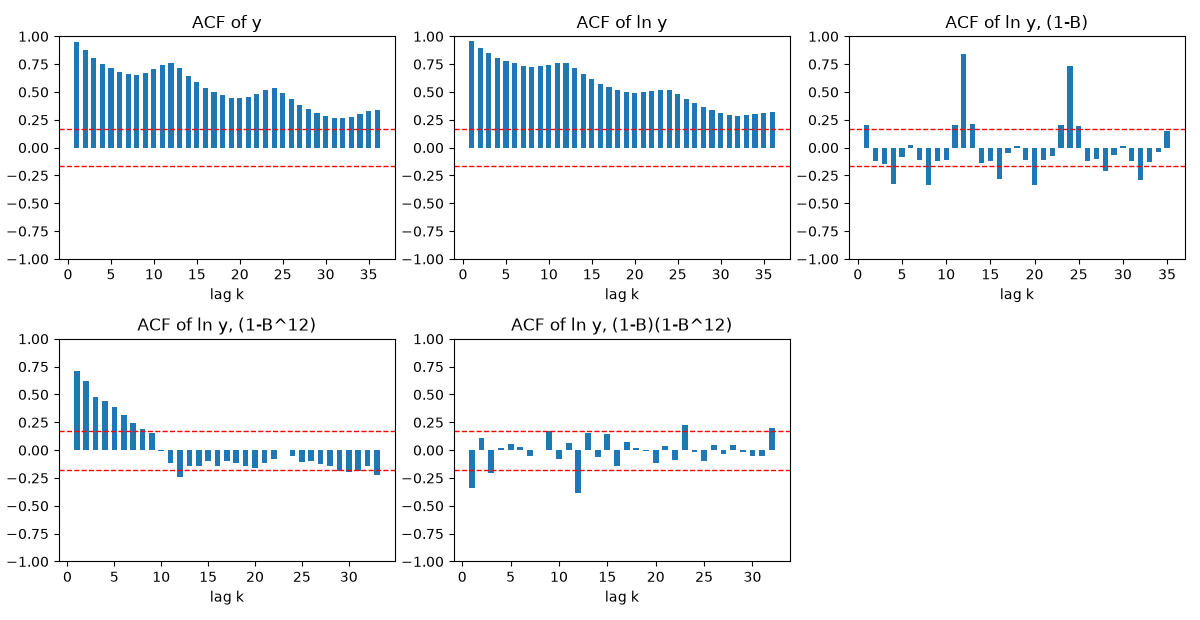
\includegraphics[width=0.98\linewidth]{fig_acf.png}

    \vspace{-0.1em}
    \raggedright\scriptsize
    Trend: slow decay. Season: spikes at lags $12,24$ after one difference.
    The mean and the yearly standard deviation both rise ($13\to62$), so the
    series is not stationary; the double difference is.\par
  \end{column}
  \end{columns}
\end{frame}

% ===================== 5. TRANSFORMATIONS ===========================
\begin{frame}{5. Stabilizing the variance: Box--Cox and log differences}
  \begin{columns}[T]
  \begin{column}{0.50\textwidth}
    \small
    $y^{(\lambda)}=\dfrac{y^\lambda-1}{\lambda\dot y^{\lambda-1}}$
    ($\lambda\ne0$), $\dot y\ln y$ ($\lambda=0$); $\dot y=255.2$.
    SSE of $y^{(\lambda)}$ on trend $+$ month:

    \vspace{0.2em}
    {\scriptsize
    \begin{tabular}{@{}llr@{}}
      \toprule
      $\lambda$ & transform & SSE \\
      \midrule
      $1$    & none        & $90{,}820$ \\
      $0.5$  & square root & $34{,}908$ \\
      $0$    & log         & $30{,}013$ \\
      $-1$   & reciprocal  & $179{,}492$ \\
      $0.20$ & grid minimum & $26{,}435$ \\
      \bottomrule
    \end{tabular}}

    \vspace{0.2em}
    $\hat\lambda=0.20$; the log is close and the standard choice. Yearly sd vs.\
    mean: corr $0.994$ (raw), $0.855$ (log). $100[\ln y_t-\ln y_{t-1}]\approx$ \% change
    (mean gap $0.57$ points).
  \end{column}
  \begin{column}{0.50\textwidth}
    \centering
    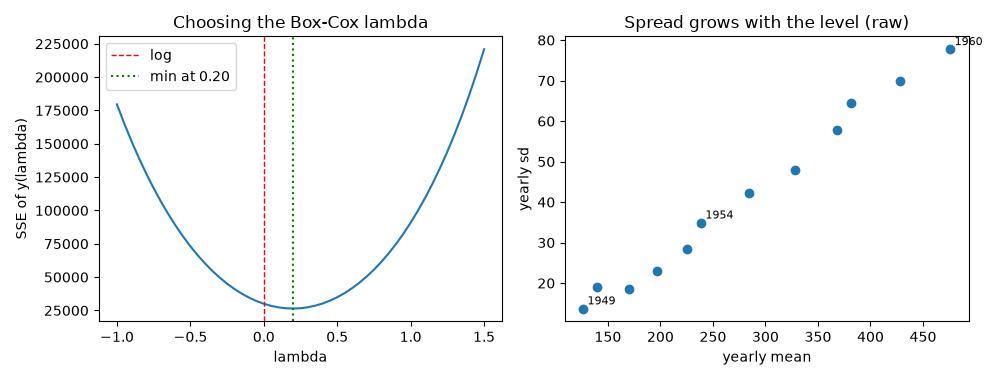
\includegraphics[width=0.98\linewidth]{fig_boxcox.png}

    \vspace{-0.1em}
    {\scriptsize Left: SSE against $\lambda$. Right: the spread grows with the level.}
  \end{column}
  \end{columns}
\end{frame}

% ===================== 6. TREND, DIFFERENCING, DECOMPOSITION ========
\begin{frame}{6. Trend, differencing and decomposition}
  \begin{columns}[T]
  \begin{column}{0.54\textwidth}
    \small
    {\scriptsize\setlength{\tabcolsep}{3pt}
    \begin{tabular}{@{}lrrr@{}}
      \toprule
      trend fit & $R^2$ & resid sd & $r_1$ of resid. \\
      \midrule
      linear (2.17)       & $0.8536$ & $46.1$ & $0.731$ \\
      quadratic (2.18)    & $0.8618$ & $44.9$ & $0.713$ \\
      exponential (2.19)  & $0.8561$ & $45.7$ & $0.723$ \\
      \bottomrule
    \end{tabular}}

    \vspace{0.2em}
    {\scriptsize Exponential: $12.1\%$ per year. A trend fit leaves
    strongly autocorrelated residuals.}

    \vspace{0.4em}
    \small
    \key{Operators.} $(1-B)^2y_t=y_t-2y_{t-1}+y_{t-2}$ (first values
    $8,-17,-5,22$) but $(1-B^2)y_t=y_t-y_{t-2}$ ($20,11,-11,6$): equal only for
    $d=1$. sd of $\ln y$: $0.442\to0.107\to0.062\to0.046$ for
    none, $(1-B)$, $(1-B^{12})$, both.

    \vspace{0.3em}
    \key{Additive or multiplicative?} Yearly range of the detrended series
    against the level: additive $46\to130$ (corr $0.87$); ratio $0.36\to0.28$
    (corr $0.13$): \emph{multiplicative}. Seasonal indices: July $1.227$,
    August $1.220$, November $0.801$.
  \end{column}
  \begin{column}{0.46\textwidth}
    \centering
    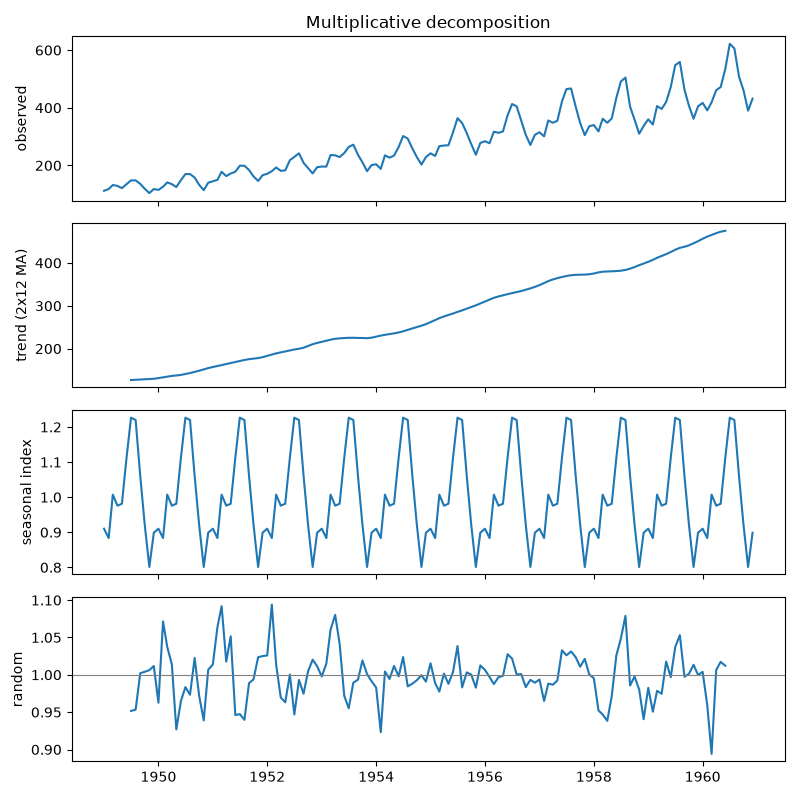
\includegraphics[width=0.86\linewidth]{fig_decomp.png}

    \vspace{-0.1em}
    {\scriptsize Slide-17 example reproduced: indices $10,-5,-8,3$ (sum $0$).}
  \end{column}
  \end{columns}
\end{frame}

% ===================== 7. ACCURACY AND ERROR CHECKS =================
\begin{frame}{7. Forecast accuracy and checking the errors}
  \begin{columns}[T]
  \begin{column}{0.56\textwidth}
    \small
    One-step-ahead errors, refitted at each of the last $24$ origins:

    \vspace{0.2em}
    {\scriptsize\setlength{\tabcolsep}{3pt}
    \begin{tabular}{@{}lrrrrr@{}}
      \toprule
       & ME & MAD & $\hat\sigma_e$ & $1.25$MAD & MAPE \% \\
      \midrule
      mean              & $190.4$ & $190.4$ & $203.4$ & $237.9$ & $40.75$ \\
      naive             & $4.0$   & $44.2$  & $51.8$  & $55.3$  & $9.73$ \\
      seasonal naive    & $47.6$  & $47.6$  & $50.0$  & $59.5$  & $10.52$ \\
      drift             & $1.4$   & $44.0$  & $51.9$  & $55.0$  & $9.70$ \\
      trend + season    & $-30.0$ & $30.0$  & $35.1$  & $37.5$  & $7.15$ \\
      trend+season+AR(1) & $-8.3$ & $15.8$  & $19.6$  & $19.7$  & $3.56$ \\
      \bottomrule
    \end{tabular}}

    \vspace{0.3em}
    \small
    $\hat\sigma_e=\sqrt{MSE}\approx1.25\,MAD$ agrees for the best model
    ($19.6$ vs.\ $19.7$). The AR(1) step on the trend-and-season residuals
    ($r_1=0.78$) removes most of the bias ($ME$ $-30\to-8$).
  \end{column}
  \begin{column}{0.44\textwidth}
    \centering
    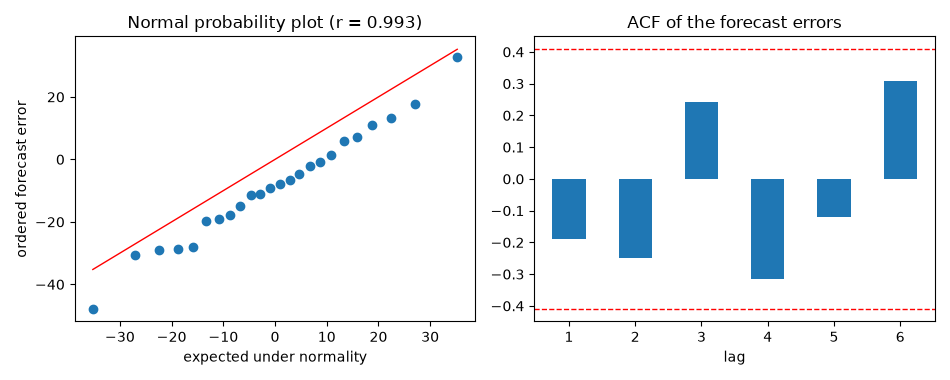
\includegraphics[width=0.98\linewidth]{fig_errdiag.png}

    \vspace{0.1em}
    \raggedright\scriptsize
    Normal: Anderson--Darling $P=0.98$, $r=0.993$. White noise: all
    $|Z_0|<1.96$; $Q_{BP}=8.73$ ($P=0.19$), $Q_{LB}=11.29$ ($P=0.08$), $6$ df.
    Only $T=24<50$ errors, so the tests have little power.\par
  \end{column}
  \end{columns}
\end{frame}

% ===================== 8. MODEL CHOICE ==============================
\begin{frame}{8. Choosing between models: AIC, SIC and a hold-out}
  \small
  Response $\ln y_t$, $T=144$; $p$ counts every estimated parameter (a monthly
  season adds $12-1=11$; a moving average estimates none):

  \vspace{0.3em}
  {\scriptsize\setlength{\tabcolsep}{3pt}
  \begin{tabular}{@{}lrrrrrr@{}}
    \toprule
    model & $p$ & $s$ & $R^2_{adj}$ & $AIC$ & $SIC$ & MSPR \\
    \midrule
    linear trend                  & $2$  & $0.1390$ & $0.9008$ & $-3.932$ & $-3.891$ & $0.0295$ \\
    linear + 1 harmonic           & $4$  & $0.0895$ & $0.9589$ & $-4.800$ & $-4.717$ & $0.0142$ \\
    linear + 2 harmonics          & $6$  & $0.0680$ & $0.9763$ & $-5.335$ & $-5.211$ & $0.0120$ \\
    linear + 11 monthly indicators & $13$ & $0.0593$ & $0.9820$ & $-5.564$ & $-5.296$ & $0.0107$ \\
    quadratic + 11 monthly indicators & $14$ & $0.0482$ & $0.9881$ & $-5.973$ & $-5.684$ & $0.0023$ \\
    \bottomrule
  \end{tabular}}

  \vspace{0.4em}
  \begin{itemize}
    \item AIC, SIC, $R^2_{adj}$ and the hold-out MSPR (fit on $120$ months,
          test on $24$) all choose the quadratic trend with monthly indicators.
    \item $AIC=\ln(\sum e_t^2/T)+2p/T$, $SIC=\ln(\sum e_t^2/T)+p\ln T/T$:
          the software value differs by a factor $T$ and the constant
          $T(\ln2\pi+1)=408.65$ for every model, so only differences matter.
    \item Plain $R^2$ always rises with $p$ ($0.9015\to0.9892$); the penalty
          did not stop here because each added term really helps.
  \end{itemize}
\end{frame}

% ===================== 9. MONITORING AND SUMMARY ====================
\begin{frame}{9. Monitoring the model, and the modelling approach}
  \begin{columns}[T]
  \begin{column}{0.50\textwidth}
    \centering
    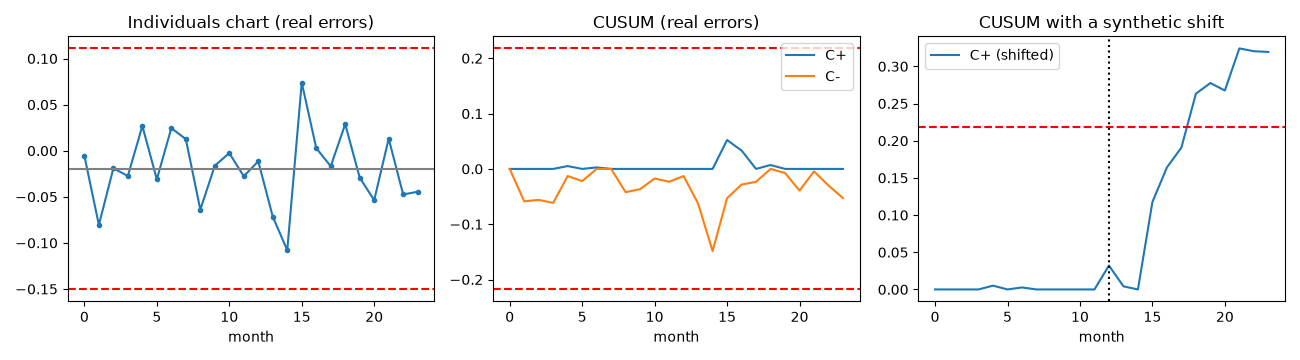
\includegraphics[width=0.98\linewidth]{fig_control.png}

    \vspace{0.2em}
    \raggedright\scriptsize
    Log-scale one-step errors: $\hat\sigma_e=0.8865\,\overline{MR}=0.0436$;
    limits $-0.151\ldots+0.111$; CUSUM $K=0.5\hat\sigma_e$, $H=5\hat\sigma_e$
    (rule of thumb, not on the slide). No alarm on the real errors; a synthetic
    $+1.5\hat\sigma_e$ shift from month $13$ is flagged after $3$ months (chart)
    and $6$ (CUSUM).\par
  \end{column}
  \begin{column}{0.50\textwidth}
    \small
    \key{The seven steps, as done here:} plot; log, then remove trend and
    season ($p=13$); model the residuals (AR(1), $r_1=0.78$); validate on the
    last $24$ months; back-transform with $\exp$; intervals on the log scale;
    monitor the one-step errors.

    \vspace{0.4em}
    \key{Takeaway.} Trend + season + AR(1) cuts the one-step MAPE to $3.6\%$
    from $9.7$--$10.5\%$ for the simple benchmarks; the errors look normal and
    uncorrelated, though $24$ observations cannot prove it.
  \end{column}
  \end{columns}
\end{frame}

\end{document}
